%\textit{•}%!TEX TS-program = xelatex

\documentclass[]{cv-class}
\usepackage{afterpage}
\usepackage{hyperref}
\usepackage{color}
\usepackage{xcolor}
\hypersetup{
    colorlinks=true,
    linkcolor=blue
}
\addbibresource{bibliography.bib}
\RequirePackage{xcolor}
\usepackage[utf8]{inputenc}
\usepackage[english]{babel} 
\usepackage[usenames, dvipsnames]{color}

\begin{document}

\begin{aside}
\color{blue}
%  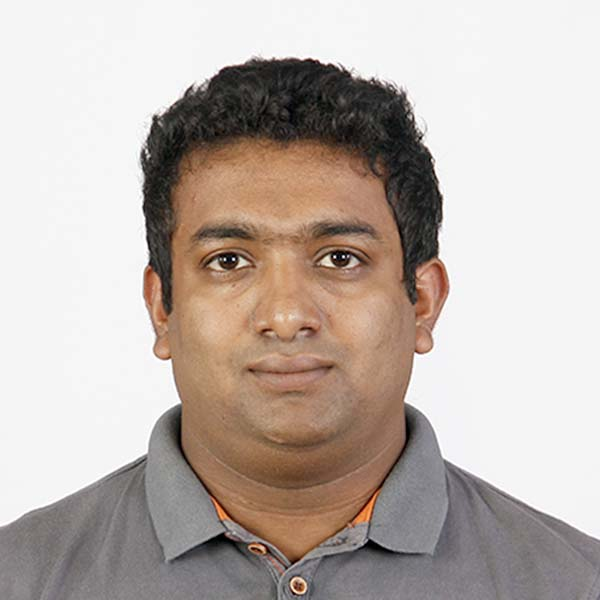
\includegraphics[scale=0.9]{img/photo.jpg}
%    ~
  \section{}
  	\vspace{0.5cm}
   ~  
  \header{Janitha}{Madushan}
      {Sr. Software Engineer}
   ~
%  \section{ADDRESS}
%    {\whitebodyfont No:04, "SunHill",\\
%    Vajirapura,\\
%    Nuwara-Eliya,\\
%    Sri-Lanka.}
%    ~
%  \section{MOBILE}
%    {\whitebodyfont +94 71 57 81 553\\
%    +94 75 97 46 502}
%    ~
  \section{MAILING}
    \underline{\href{mailto:janithasen@gmail.com}{{\whitebodyfont janithasen@gmail.com}}}
    ~
%  \section{LANGAUGES}
%  	{\whitebodyfont Sinhalese (Native)\\
%    Engilsh}
%    ~ 
%  \section{NIC}
%  	{\whitebodyfont 901540160V}
%    ~
%  \section{BIRTHDAY}
%  	{\whitebodyfont June 02,1990}
%    ~
  \section{WEB}
  	\vspace{0.10cm}
    \underline{\href{https://www.linkedin.com/in/janithamadushan}{{\whitebodyfont Linkedin}}}
    \\
	\vspace{0.10cm}
    \underline{\href{https://stackoverflow.com/users/4412223/janitha-madushan}{{\whitebodyfont Stackoverflow}}}
	\\	
	\vspace{0.10cm}
    \underline{\href{https://github.com/janitham}{{\whitebodyfont Github}}}
    ~
  \section{OS}
    \asidelist{{\whitebodyfont Windows}}
    {\includegraphics[scale=0.30]{img/star.png}
    \includegraphics[scale=0.30]{img/star.png}
    \includegraphics[scale=0.30]{img/star.png}
    \includegraphics[scale=0.30]{img/star.png}
    \includegraphics[scale=0.30]{img/star.png}}
    \asidelist{\whitebodyfont{Linux}}
    {\includegraphics[scale=0.30]{img/star.png}
    \includegraphics[scale=0.30]{img/star.png}
    \includegraphics[scale=0.30]{img/star.png}
    \includegraphics[scale=0.30]{img/star.png}
    \includegraphics[scale=0.30]{img/star_empty.png}}
    ~
  \section{LANGUAGES}
    \asidelist{{\whitebodyfont Java}}
    {\includegraphics[scale=0.30]{img/star.png}
    \includegraphics[scale=0.30]{img/star.png}
    \includegraphics[scale=0.30]{img/star.png}
    \includegraphics[scale=0.30]{img/star.png}
    \includegraphics[scale=0.30]{img/star.png}}
    \asidelist{\whitebodyfont{JavaScript}}
    {\includegraphics[scale=0.30]{img/star.png}
    \includegraphics[scale=0.30]{img/star.png}
    \includegraphics[scale=0.30]{img/star.png}
    \includegraphics[scale=0.30]{img/star.png}
    \includegraphics[scale=0.30]{img/star_empty.png}}
	\asidelist{\whitebodyfont{Pyhon}}
    {\includegraphics[scale=0.30]{img/star.png}
    \includegraphics[scale=0.30]{img/star.png}
    \includegraphics[scale=0.30]{img/star.png}
    \includegraphics[scale=0.30]{img/star.png}
    \includegraphics[scale=0.30]{img/star_empty.png}}
    \asidelist{\whitebodyfont{C}}
    {\includegraphics[scale=0.30]{img/star.png}
    \includegraphics[scale=0.30]{img/star.png}
    \includegraphics[scale=0.30]{img/star.png}
    \includegraphics[scale=0.30]{img/star.png}
    \includegraphics[scale=0.30]{img/star.png}}
    ~
  \section{TECHNOLOGIES}
    \asidelist{{\whitebodyfont Spring}}
    {\includegraphics[scale=0.30]{img/star.png}
    \includegraphics[scale=0.30]{img/star.png}
    \includegraphics[scale=0.30]{img/star.png}
    \includegraphics[scale=0.30]{img/star.png}
    \includegraphics[scale=0.30]{img/star.png}}
    \asidelist{\whitebodyfont{Hibernate}}
    {\includegraphics[scale=0.30]{img/star.png}
    \includegraphics[scale=0.30]{img/star.png}
    \includegraphics[scale=0.30]{img/star.png}
    \includegraphics[scale=0.30]{img/star.png}
    \includegraphics[scale=0.30]{img/star.png}}
    \asidelist{\whitebodyfont{Docker}}
    {\includegraphics[scale=0.30]{img/star.png}
    \includegraphics[scale=0.30]{img/star.png}
    \includegraphics[scale=0.30]{img/star.png}
    \includegraphics[scale=0.30]{img/star.png}
    \includegraphics[scale=0.30]{img/star_empty.png}}
	\asidelist{\whitebodyfont{Kubernetes}}
    {\includegraphics[scale=0.30]{img/star.png}
    \includegraphics[scale=0.30]{img/star.png}
    \includegraphics[scale=0.30]{img/star.png}
    \includegraphics[scale=0.30]{img/star.png}
    \includegraphics[scale=0.30]{img/star_empty.png}}    
    \asidelist{\whitebodyfont{Jenkins}}
    {\includegraphics[scale=0.30]{img/star.png}
    \includegraphics[scale=0.30]{img/star.png}
    \includegraphics[scale=0.30]{img/star.png}
    \includegraphics[scale=0.30]{img/star.png}
    \includegraphics[scale=0.30]{img/star.png}}
    \asidelist{\whitebodyfont{VSphere}}
    {\includegraphics[scale=0.30]{img/star.png}
    \includegraphics[scale=0.30]{img/star.png}
    \includegraphics[scale=0.30]{img/star.png}
    \includegraphics[scale=0.30]{img/star.png}
    \includegraphics[scale=0.30]{img/star_empty.png}}
    \asidelist{\whitebodyfont{AWS}}
    {\includegraphics[scale=0.30]{img/star.png}
    \includegraphics[scale=0.30]{img/star.png}
    \includegraphics[scale=0.30]{img/star.png}
    \includegraphics[scale=0.30]{img/star.png}
    \includegraphics[scale=0.30]{img/star_empty.png}}
    \asidelist{\whitebodyfont{GIT}}
    {\includegraphics[scale=0.30]{img/star.png}
    \includegraphics[scale=0.30]{img/star.png}
    \includegraphics[scale=0.30]{img/star.png}
    \includegraphics[scale=0.30]{img/star.png}
    \includegraphics[scale=0.30]{img/star_empty.png}}
    \asidelist{\whitebodyfont{Ansible}}
    {\includegraphics[scale=0.30]{img/star.png}
    \includegraphics[scale=0.30]{img/star.png}
    \includegraphics[scale=0.30]{img/star.png}
    \includegraphics[scale=0.30]{img/star_empty.png}
    \includegraphics[scale=0.30]{img/star_empty.png}}
    \asidelist{\whitebodyfont{Terraform}}
    {\includegraphics[scale=0.30]{img/star.png}
    \includegraphics[scale=0.30]{img/star.png}
    \includegraphics[scale=0.30]{img/star.png}
    \includegraphics[scale=0.30]{img/star_empty.png}
    \includegraphics[scale=0.30]{img/star_empty.png}}
    ~
      ~
  \section{DATABASES}
    \asidelist{{\whitebodyfont MySql}}
    {\includegraphics[scale=0.30]{img/star.png}
    \includegraphics[scale=0.30]{img/star.png}
    \includegraphics[scale=0.30]{img/star.png}
    \includegraphics[scale=0.30]{img/star.png}
    \includegraphics[scale=0.30]{img/star_empty.png}}
    \asidelist{\whitebodyfont{MsSql}}
    {\includegraphics[scale=0.30]{img/star.png}
    \includegraphics[scale=0.30]{img/star.png}
    \includegraphics[scale=0.30]{img/star.png}
    \includegraphics[scale=0.30]{img/star.png}
    \includegraphics[scale=0.30]{img/star_empty.png}}
	\asidelist{\whitebodyfont{Oracle}}
    {\includegraphics[scale=0.30]{img/star.png}
    \includegraphics[scale=0.30]{img/star.png}
    \includegraphics[scale=0.30]{img/star.png}
    \includegraphics[scale=0.30]{img/star_empty.png}
    \includegraphics[scale=0.30]{img/star_empty.png}}    
    ~
\end{aside}

\section{EDUCATION}
\begin{entrylist}
  \entry
    {Aug. 11 - June 15}
    {Computer Engineering}
    {Faculty of Engineering, University of Peradeniya}
    {Bsc. Computer Engineering at Faculty of Engineering of University of Peradeniya.}
\end{entrylist}

\section{EXPERIENCE}
\begin{entrylist}
  \entry
    {Nov. 15 - Now}
    {Senior Software Engineer}
    {Cambio Software Engineering}
    {Working as a Senior Software Engineer in Product development and DevOps teams. Cambio Software Engineering is committed to define and build the e-health generation. "Cambio" is the first company to have developed a platform, "Cambio Spider", that makes it possible to integrate all IT-support in a health-care organization. I worked in a very challenging environment because I had to research a lot and complete the tasks in the limited time given. In that tasks I used various technologies and strategies. \\I developed applications using \textbf{Java, Spring, Hibernate, EJB, AngularJs, Junit, Mokito, MsSql, MySql} and various latest technologies. Also I exposed to many "DevOps" technologies in this period \textbf{(Docker, Kubernetes, Maven-plugins, Maven, Jenkins, Nexus, Git, Subversion, SonarQube)}.}
\\
  \entry
    {Oct. 15 - Mar.16}
    {Internship}
    {IFS R\&D}
    {I developed one internal application and one research on "Oracle Application Express". Technologies I used in that period are \textbf{ASP.NET, ORACLE 11G/12C, PL-SQL, ORACLE-APEX, Android and Java}.}
\end{entrylist}

\section{PROJECTS}
\begin{entrylist}
	\entry
    {}
	{Snooper}    
    {Delivery Information Management Application}
	{This is a sub-project of "Stacker" project. This application stores the delivery information using a trigger from "Stacker" tool through it's RestfulAPI and graphically represents information using "AngularJs" based front end application. Backend has implemented Spring-Cloud based micro-services. \\"Redis" implementation used as Hibernate 2nd Level caching. "Elastic Search", "Logstash" \& "Kibana" integration(ELK) is used to monitor the logs, "Grafana" \& "Prometheus" integration used to monitor the states of the application. Application containerized using "Docker", "Docker-maven-plugin", Jenkins \& Jenkinsfile used to build the application. Docker-Compose is used to deploy the application. \textbf{(Java-8, Spring-cloud, Spring-boot, zuul-proxy, Hibernate, AngularJs, Docker, Docker-Compose, Gulp, Micro-Services, SpringJunit, SonarQube, MySql, Redis, Jenkins, Jenkinsfile, Kibana, Logstash, Elastic-search, Prometheus, Grafana, Git  Linux)}}
	\\
	\entry
    {}
	{Stacker}    
    {Delivery Automation Tool}
	{This is a maven-plugin which generates multi-modules pom structure using BOM(Baseline POM) and MetaData(Artifact) according to different types of 			modules in the BOM(Dependencies). The rest is done by the maven-plugins have configured in the POMs. This main plugin is configured in a Jenkins Job 		and all of plugins have released to nuxus. \textbf{(Java-8, Maven-plugins, Jenkins, Jenkins-pipelines, Junit, Mokito, SonarQube)}}
	\end{entrylist}
\newpage
\begin{aside}
\end{aside}

\begin{entrylist}
\entry
    {}
	{ART}    
    {Delivery Application}
{This is a web based delivery application which generates specific pom structure is used inside the company based on BOM(Baseline POM). The application consists a database which holds necessary data. The application is integrated with AD and roles are saved inside the application since this is a role based application. \textbf{(JAVA-8, Spring, Spring-Security, Hibernate, AngularJs, JBoss, SOA, MSSQL, T-SQL, Junit, Mokito, SonarQube)}}
\\
  	\entry
    {}
    {IFS Rest Data Service}
    {Internship Project}
    {Research on exposing database as  RESTful  services. Demonstrated  using  MS  excel  office  application. \textbf{(ORACLE 12/C, PL-SQL, ORACLE-APEX, OFFICE-APPS)}}
	\\
\end{entrylist}



\section{CERTIFICATIONS}
\begin{entrylist}
\entry
    {}
	{1ZO-809}
    {}
	{Oracle Certified Associate, Java SE 8 Programmer}
\\
\entry
    {}
	{AWS}
    {}
	{AWS Certified Solutions Architect Associate}
\end{entrylist}


\section{ASSOCIATIONS}
\begin{entrylist}
\entry
    {}
	{IESL}    
    {}
	{Associate Member of Institute of Engineers Sri Lanka}
\end{entrylist}
\begin{entrylist}
  \entry
    {}
    {}
    {}
    {\textbf{References available upon request}}
  \entry
    {}
    {}
    {}
    {I do here by certify that above particulars are true and correct. If you are pleased to consider me suitable for your company and select me as an employee, it will be my earnest endeavor to discharge the duties entrusted to me, to the best of my ability and rise to your expectations.}
\end{entrylist}

\begin{flushright}
\emph{\textbf{Janitha Madushan}}
\end{flushright}
\begin{flushright}
\emph{\textbf{\today}}
\end{flushright}

\end{document}